\section{User Interface}
\label{sec:chapter_2_section_4}

Qui si fa una descrizione della User Interface...

\subsection{Viewer 2D}
The \emph{2D-viewer} invokes the \emph{2Dgf} of the building elements added to the model and renders its output using SVG elements. To cope with frequent updates coming from the user drawing interaction, it exploits the \emph{Virtual DOM}~\cite{vdom}, which permits to update only the modified part thus avoiding complete redrawing of the scene. To perform pan and zoom operations, typically necessary in this kind of tool, we develop an ad-hoc React component named \emph{ReactSVGPanZoom}\footnote{https://github.com/chrvadala/react-svg-pan-zoom}.
\begin{figure}[htbp] %  figure placement: here, top, bottom, or page
   \centering
   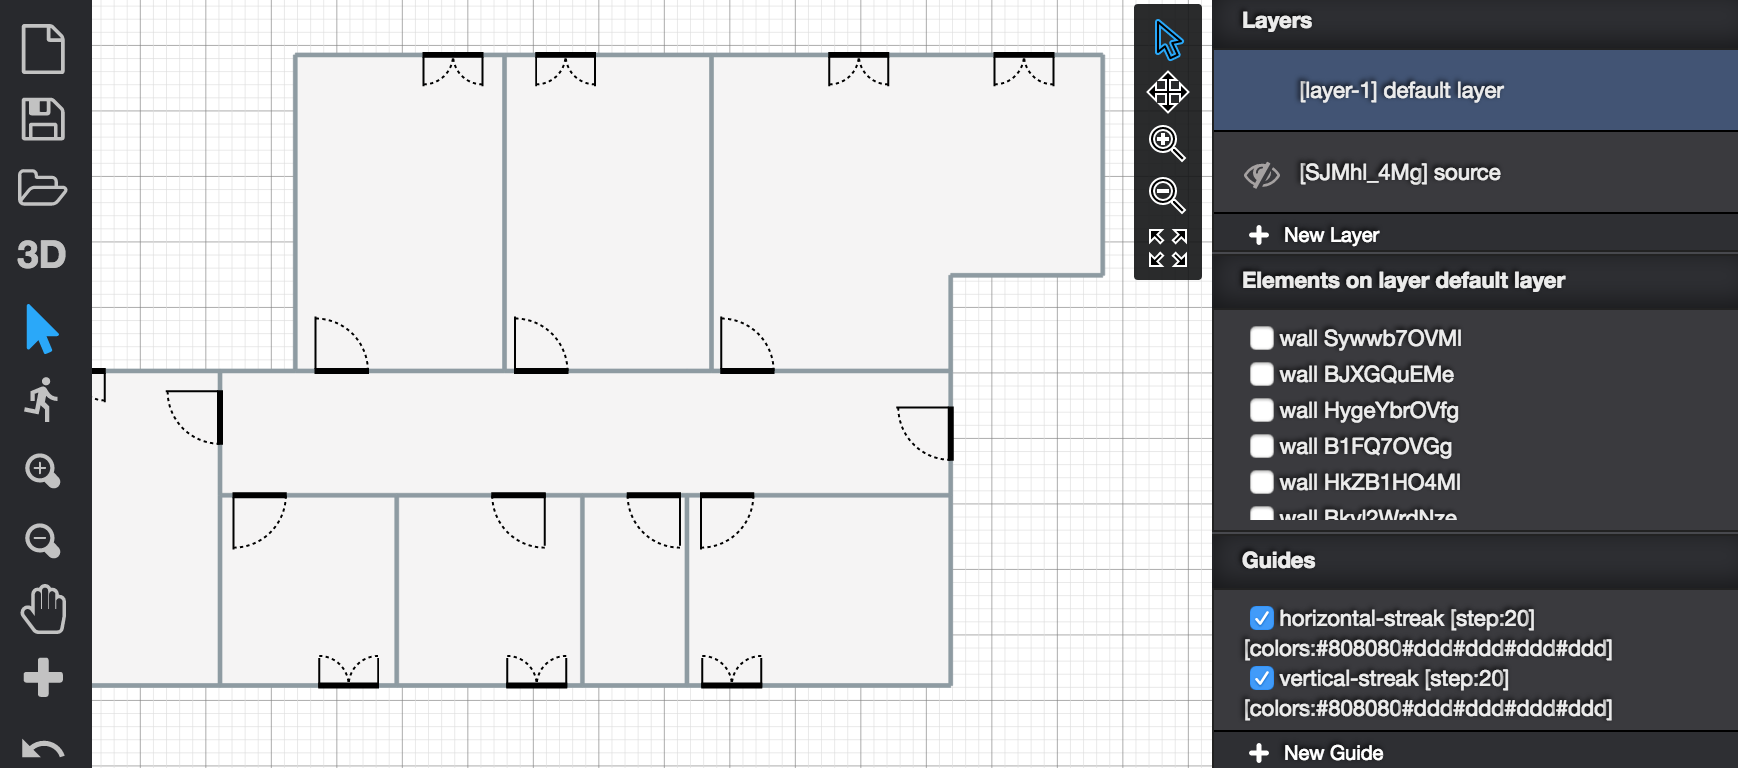
\includegraphics[width=1\linewidth]{images/2d}
   \caption{Schermata viewer 2D}
   \label{fig:view2D}
\end{figure}
   (see Figure~\ref{fig:view2D})
   \newpage


\subsection{Viewer 3D}
The \emph{3D-viewer} invokes the \emph{3Dgf} of the building elements added to the model and renders its output using WebGL primitives via \emph{Three.js}~\footnote{https://threejs.org/}. It has been implemented a \emph{diff} and \emph{patch} system, standardized in~\cite{rfc6902}: Three.js objects are associated with building elements inside the state, so every time the user triggers an action that results in a state alteration, the application computes the difference between the old state and the new one and changes only the affected object. In particular we can have the following \textit{operations}: (i) \emph{add}, (ii) \emph{replace} and (iii) \emph{remove}.
\begin{figure}[htbp] %  figure placement: here, top, bottom, or page
   \centering
   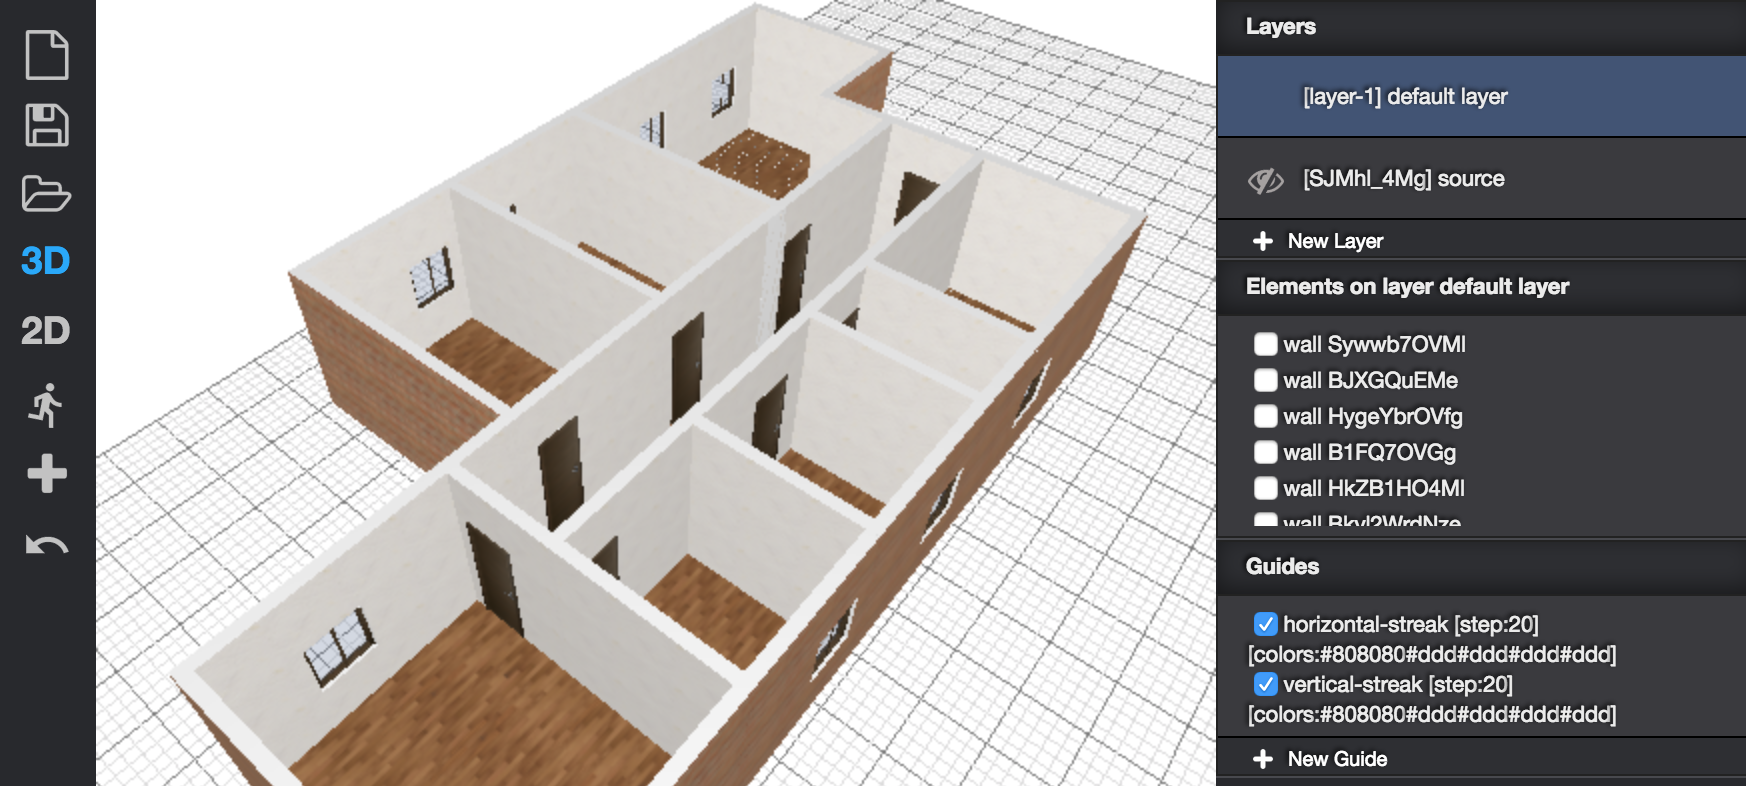
\includegraphics[width=1\linewidth]{images/3d}
   \caption{Schermata viewer 3D }
   \label{fig:viewer3D}
\end{figure}
   (see Figure~\ref{fig:viewer3D})
   \newpage
